\documentclass[aspectratio=169]{beamer}
\usetheme{Boadilla}
\usecolortheme{seahorse}
\usepackage[T1]{fontenc}
\usepackage{lmodern}
\usepackage{booktabs}
\usepackage{amsmath}
\usepackage{xcolor}
\usepackage{tikz}
\usetikzlibrary{arrows.meta,positioning}

\setbeamertemplate{navigation symbols}{}
\setbeamertemplate{itemize items}[circle]

\newcommand{\shapebox}[2]{%
  \begin{center}
  \colorbox{black!8}{\parbox{0.9\textwidth}{\centering
  \textbf{IN:} \texttt{#1} \qquad$\longrightarrow$\qquad \textbf{OUT:} \texttt{#2}}}
  \end{center}}

\title{How Audio Becomes a Transcript}
\subtitle{What \texttt{run\_whisperx.py} accomplishes, step by step}
\author{PSYCH-ASR --- Stage 1}
\date{}

\begin{document}

\frame{\titlepage}

%----------------------------------------------------------
\begin{frame}{The whole file is five calls}

\begin{center}
\scriptsize
\begin{tabular}{llll}
\toprule
\textbf{Call} & \textbf{Question it answers} & \textbf{In} & \textbf{Out} \\
\midrule
\texttt{load\_audio} & What are the numbers? & file & \texttt{(N,)} \\
\texttt{transcribe} & What words were said? & \texttt{(N,)} & text, per chunk \\
\texttt{align} & \emph{When} was each word said? & text + \texttt{(N,)} & word times \\
\texttt{diarize} + \texttt{assign} & \emph{Who} said it? & \texttt{(N,)} & speaker labels \\
\texttt{render} & Can a human read it? & transcript & a \texttt{.txt} play script \\
\bottomrule
\end{tabular}
\end{center}

\vspace{0.2em}
\begin{center}
\resizebox{\textwidth}{!}{%
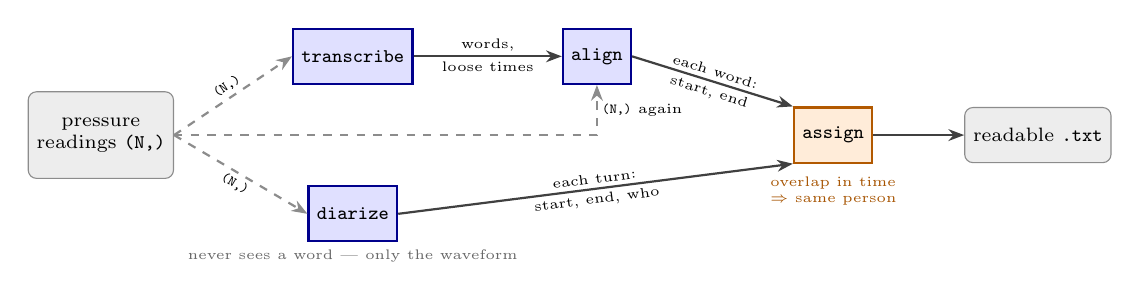
\begin{tikzpicture}[
  font=\scriptsize,
  >={Stealth[length=2mm]},
  data/.style={draw=black!45, rounded corners=3pt, fill=black!7,
               align=center, inner sep=3pt, minimum height=7mm},
  model/.style={draw=blue!55!black, thick, fill=blue!12,
                align=center, inner sep=3pt, minimum height=7mm},
  merge/.style={draw=orange!70!black, thick, fill=orange!15,
                align=center, inner sep=3pt, minimum height=7mm},
  flow/.style={->, thick, draw=black!75},
  bus/.style={->, thick, draw=black!45, dashed},
  lbl/.style={font=\tiny, inner sep=1.5pt}
]

\node[data, minimum height=11mm] (A) at (0,0) {pressure\\readings \texttt{(N,)}};
\node[model] (T)  at (3.2,1.0)  {\texttt{transcribe}};
\node[model] (AL) at (6.3,1.0)  {\texttt{align}};
\node[model] (D)  at (3.2,-1.0) {\texttt{diarize}};
\node[merge] (AS) at (9.3,0)    {\texttt{assign}};
\node[data]  (R)  at (11.9,0)   {readable \texttt{.txt}};

% the audio bus: all three models re-read the SAME array
\draw[bus] (A.east) -- node[lbl, above, sloped] {\texttt{(N,)}} (T.west);
\draw[bus] (A.east) -- node[lbl, below, sloped] {\texttt{(N,)}} (D.west);
\draw[bus] (A.east) -- (6.3,0) -- node[lbl, right] {\texttt{(N,)} again} (AL.south);

% text moving forward
\draw[flow] (T) -- node[lbl, above] {words,}
                   node[lbl, below] {loose times} (AL);
\draw[flow] (AL.east) -- node[lbl, above, sloped] {each word:}
                         node[lbl, below, sloped] {start, end} (AS.north west);
\draw[flow] (D.east) -- node[lbl, above, sloped] {each turn:}
                        node[lbl, below, sloped] {start, end, who} (AS.south west);
\draw[flow] (AS) -- (R);

\node[lbl, text=black!60, below=1pt of D] {never sees a word --- only the waveform};
\node[lbl, text=orange!65!black, below=3pt of AS, align=center]
      {overlap in time\\$\Rightarrow$ same person};
\end{tikzpicture}}
\end{center}

{\scriptsize Dashed = the \emph{same} array, read from scratch three times --- the models
share no internals. Solid = text moving forward.}

\end{frame}

%----------------------------------------------------------
\begin{frame}{Step 1 --- \texttt{load\_audio}: sound becomes numbers}

\shapebox{audio file (.wav)}{float32 array, (N,)}

A microphone measures \textbf{air pressure}. 16{,}000 times per second we write down the
current pressure as a number between $-1$ and $1$. That flat list of $N$ numbers \emph{is}
the audio --- everything downstream reads it.

\vspace{0.8em}
\[
N = \texttt{seconds} \times 16000
\qquad\Longrightarrow\qquad
\text{50-minute session} = 48{,}000{,}000
\]

\vspace{0.5em}
\textbf{The one trick to remember:} time converts to position by multiplying by 16000. A
word starting at 4.5 seconds begins at index $72{,}000$. Every timestamp in this pipeline
is ultimately a statement about where you are in this array.

\end{frame}

%----------------------------------------------------------
\begin{frame}{Step 2 --- \texttt{transcribe}, part 1: audio becomes a picture}

\shapebox{(N,)}{one picture per 30-second chunk}

One call doing five jobs. The first three just get the audio into a shape the model can eat:

\begin{itemize}
  \item \textbf{Find the speech.} A small model marks speech vs.\ silence. It transcribes
        nothing --- it only draws boundaries.
  \item \textbf{Pack into chunks.} Whisper only ever swallows 30 seconds at a time --- that
        is the size of its mouth and it never changes. So speech stretches get taped
        end-to-end until the next one would push past 30 seconds; then a new chunk starts.
        \textbf{Nothing about the conversation decides where that cut lands} --- only the
        30-second ceiling does. Chunks do not depend on each other, so 16 can go through the
        GPU at once. That is \texttt{batch\_size}.
  \item \textbf{Turn each chunk into a picture.} A spectrogram: time along one axis, pitch
        along the other, brightness = how much of that pitch is present.
\end{itemize}

\end{frame}

%----------------------------------------------------------
\begin{frame}{Step 2 --- \texttt{transcribe}, part 2: picture becomes words}

\shapebox{one picture per chunk}{segments of text}

The other two jobs are the two neural halves of Whisper:

\begin{itemize}
  \item \textbf{The encoder reads the picture.} A 20 ms sliver of sound means nothing by
        itself --- the same buzz sits inside ``said'' and ``sat'', and only the sound around
        it settles which. So every sliver gets to look at every other sliver in the 30
        seconds and rewrite itself with that context. That looking-around is
        \textbf{self-attention}, and a sliver 25 seconds away is just as easy to reach as
        the one next door. Do it enough times and each sliver describes its moment
        \emph{in the context of the whole chunk}.
  \item \textbf{The decoder writes the words}, one token at a time, like a chatbot: predict,
        append, predict again --- reading the encoder's output as it goes, because that is
        the only channel through which the audio reaches it.
\end{itemize}

\end{frame}

%----------------------------------------------------------
\begin{frame}{What \texttt{transcribe} hands back}

\begin{center}
\small
\begin{tabular}{rlll}
\toprule
\textbf{start} & \textbf{end} & \textbf{text} & \textbf{avg\_logprob} \\
\midrule
0.0 & 26.0 & ``so how has this week been for you \dots'' & $-0.09$ \\
27.0 & 55.0 & ``I guess it started okay but then \dots'' & $-0.14$ \\
\bottomrule
\end{tabular}
\end{center}

\vspace{0.8em}
\textcolor{red}{\textbf{Read those timestamps carefully.}} They are \emph{chunk boundaries}
--- artifacts of the 30-second packing. They are not sentence boundaries, and they were
never measured from the speech.

\vspace{0.5em}
\textbf{Not one individual word has a timestamp yet.} Each segment is one undifferentiated
string. That hole is the entire reason the next step exists.

\vspace{0.3em}
{\small(\texttt{avg\_logprob} is the model's confidence, and Stage 2's quality triage runs on
it. Above $-0.5$ is a confident decode; below $-1.0$ is where hallucination starts.)}

\end{frame}

%----------------------------------------------------------
\begin{frame}{Step 3 --- \texttt{align}: this is karaoke}

\shapebox{segments + (N,)}{segments, each with a "words" list}

\textbf{Karaoke never guesses the lyrics.} It was handed them. All it decides is which word
lights up at which moment.

\vspace{0.5em}
That is this step. \texttt{transcribe} gave us the words but not their times, so a smaller
model (\texttt{wav2vec2}) listens to the raw audio again and walks the known words against
it in order.

\vspace{0.4em}
\textbf{Because the words are handed to it, it cannot make any up} --- it cannot skip, add,
or reorder. It only decides where each word sits on the clock.

\begin{center}
\scriptsize
\begin{tabular}{lrrr}
\toprule
\textbf{word} & \textbf{start} & \textbf{end} & \textbf{score} \\
\midrule
so & 0.31 & 0.44 & 0.91 \\
how & 0.46 & 0.63 & 0.88 \\
has & 0.65 & 0.79 & 0.94 \\
\bottomrule
\end{tabular}
\end{center}

\vspace{0.2em}
Now we know \textbf{what} was said and \textbf{when}. Still no idea \textbf{who} said it.
{\small (Side effect: segments come back re-split at sentence boundaries, so the segment
count goes \emph{up}.)}

\end{frame}

%----------------------------------------------------------
\begin{frame}{Step 4 --- \texttt{diarize}: whose voice is this?}

\begin{center}
\colorbox{red!12}{\parbox{0.92\textwidth}{\centering
\textbf{Diarization does not use the Whisper \emph{model}.} \\[0.3em]
\footnotesize The class lives in \texttt{whisperx.diarize}, but that file is a thin wrapper
--- every model it runs comes from \texttt{pyannote}. It never sees the transcript or the
words; it starts over from the raw \texttt{(N,)} array.}}
\end{center}

\vspace{0.3em}
Whisper asked what sounds were made. This asks who made them --- and you can tell two
strangers apart in a language you do not speak. It takes three moves.

\vspace{0.8em}
\textbf{Move one: find the talking.} Mark every stretch where somebody is speaking --- and
every stretch where \textbf{two people are speaking at once}.

\vspace{0.5em}
Spotting an overlap needs no idea \emph{who} is talking. Two tangled voices simply sound
different from one, the way you can hear that a room is crowded without recognising a single
person in it.

\vspace{0.5em}
Overlapping stretches sit out the next move, because a smear of two voices describes neither
of them. \textbf{Nothing is deleted} --- Whisper transcribed those words long ago and they
stay in the transcript.

\end{frame}

%----------------------------------------------------------
\begin{frame}{Move two --- turn each voice into numbers}

\shapebox{one stretch of speech}{a list of 256 numbers}

A second model listens to one clean stretch and turns it into a list of \textbf{256
numbers}. Always 256 --- whether the stretch ran one second or twenty.

\vspace{0.6em}
\textbf{Why numbers?} Because two voices cannot be compared directly, but two lists of
numbers can.

\vspace{0.6em}
The model was trained on thousands of speakers with one rule: two clips of the \emph{same}
person must come out with similar numbers, two clips of \emph{different} people far apart.
It was never taught a single word.

\vspace{0.6em}
So what survives in those 256 numbers is the \textbf{voice} --- pitch, resonance,
breathiness --- and nothing about what was said. A muttered ``mm-hm'' and a two-minute story
from the same person still come out looking alike.

\end{frame}

%----------------------------------------------------------
\begin{frame}{Move three --- cluster, and what comes back}

\textbf{Cluster.} Sort the 256-number fingerprints into piles by how close together they
sit. Each pile is one speaker, and every stretch in that pile gets its label:

\begin{center}
\small
\begin{tabular}{rrl}
\toprule
\textbf{start} & \textbf{end} & \textbf{speaker} \\
\midrule
0.3 & 3.9 & SPEAKER\_00 \\
4.1 & 9.5 & SPEAKER\_01 \\
9.8 & 14.8 & SPEAKER\_00 \\
\bottomrule
\end{tabular}
\end{center}

\vspace{0.5em}
Times and speakers. \textbf{No words anywhere.} This table has never seen the transcript.

\vspace{0.5em}
\textbf{Why we pass \texttt{-{}-num-speakers 2}.} Left alone, clustering guesses the number
of groups and errs both ways: it splits one person in two when their voice shifts (calm
vs.\ distressed patient), and merges two people whose voices are similar. Every pilot
session has exactly two people in it, so we say so and remove both failure modes.

\vspace{0.3em}
Labels are arbitrary --- \texttt{SPEAKER\_00} is not the therapist. Mapping labels to roles
is Stage 2's first job.

\end{frame}

%----------------------------------------------------------
\begin{frame}{Step 5 --- \texttt{assign}: stack the two lists}

We now hold two lists built in total ignorance of each other, sharing exactly one thing:
\textbf{a clock}. \texttt{align} says \emph{which word} happened when. \texttt{diarize} says
\emph{who was talking} when. Lay one on top of the other and read the answer off.

For each word, look at whose stretch it lands inside; if it straddles a handover, whoever
covers more of it wins:

\begin{center}
\scriptsize
\begin{tabular}{lccl}
\toprule
turn & span & overlap with ``okay'' (3.0--3.4) & \\
\midrule
SPEAKER\_00 & 0.0--3.1 & 0.1 s & \\
SPEAKER\_01 & 3.1--8.0 & \textbf{0.3 s} & $\leftarrow$ winner \\
\bottomrule
\end{tabular}
\end{center}

\vspace{0.3em}
\textbf{This is why alignment had to run first.} Without it we are not placing a word, we
are placing a 26-second chunk --- and half a minute of dialogue gets stamped onto whoever
dominated it.

\end{frame}

%----------------------------------------------------------
\begin{frame}{Step 6 --- \texttt{render}: nobody wants to read JSON}

\shapebox{transcript with speakers}{\texttt{<stem>.transcript.txt}}

The check this whole project hinges on is a \textbf{human} listening to the audio with the
transcript open. That person needs a play script, not a data structure. One more pass ---
pure formatting, no model, CPU, sub-second --- groups consecutive segments sharing a speaker
into one block and prints it:

\begin{center}
\colorbox{black!8}{\parbox{0.88\textwidth}{\ttfamily\small
[00:00] SPEAKER\_00 \\
\hspace*{2em}So how was the week? \\[0.3em]
[00:04] SPEAKER\_01 \\
\hspace*{2em}It was rough. I did not leave the house Tuesday. \\[0.3em]
[00:15] UNKNOWN \\
\hspace*{2em}Mm-hm.
}}
\end{center}

\vspace{0.3em}
Grouping matters because alignment re-split everything at sentence boundaries --- ungrouped,
a minute of speech reads as a list of sentences, not a conversation. \texttt{UNKNOWN} is
printed rather than hidden: a cluster of them \emph{is} the finding.

\end{frame}

%----------------------------------------------------------
\begin{frame}{End to end}

\begin{center}
\small
\begin{tabular}{lll}
\toprule
\textbf{Step} & \textbf{In} & \textbf{Out} \\
\midrule
\texttt{load\_audio} & audio file & \texttt{(N,)} float32 \\
\texttt{transcribe} & \texttt{(N,)} & segments: text + chunk bounds \\
\texttt{align} & segments + \texttt{(N,)} & segments + per-word start/end/score \\
\texttt{DiarizationPipeline} & \texttt{(N,)} & turns table: start, end, speaker \\
\texttt{assign\_word\_speakers} & turns + transcript & \texttt{speaker} on words/segments \\
\texttt{render\_transcript} & labelled transcript & grouped, timestamped \texttt{.txt} \\
\bottomrule
\end{tabular}
\end{center}

\vspace{1em}
Three models, one waveform read three times, joined at the end on nothing but timestamps.

\end{frame}

%----------------------------------------------------------
\begin{frame}{It all lands in \texttt{word\_segments}}

Everything above collapses into one key of
\texttt{data/stage1/<stem>.diarized.json}: a flat list, \textbf{one entry per word}, where
each entry answers every question the pipeline was built to ask.

\begin{center}
\small
\begin{tabular}{llll}
\toprule
\textbf{field} & \textbf{answers} & \textbf{came from} & \textbf{example} \\
\midrule
\texttt{word} & what was said & \texttt{transcribe} & ``okay'' \\
\texttt{start}, \texttt{end} & when & \texttt{align} & 3.02, 3.41 \\
\texttt{score} & how sure we are of the timing & \texttt{align} & 0.88 \\
\texttt{speaker} & who said it & \texttt{diarize} + \texttt{assign} & \texttt{SPEAKER\_01} \\
\bottomrule
\end{tabular}
\end{center}

\vspace{0.35em}
\textbf{That is the whole deliverable.} Every Stage 3 feature --- talk-time ratio, turn
counts, speech rate, silence, interruptions, who asked what --- is arithmetic over this one
list. (\texttt{segments} is the same content re-grouped into sentences for reading;
\texttt{language} is \texttt{"en"}.)

\vspace{0.5em}
First pilot session: \textbf{7{,}298 words}, of which 7{,}293 carry all five fields and 5
have no \texttt{speaker} --- those five landed in moments diarization had written off as
silence, and there is no fallback guess, so the field is missing. Whether the other 7{,}293
labels are \emph{correct} is the human check nothing downstream should be built before.

\end{frame}

\end{document}
